\chapter{Implementación}
En esta sección se detalla la implementación de la propuesta de solución, que se dividió en dos componentes principales. Primero, se implementó un sistema de inferencia para type-based declassification. Segundo, se elaboró un plugin para editores de texto que integra el resultado de la inferencia.

\section{Lenguaje Dart}
Dart es un lenguaje de programación de propósito general, orientado a objetos y de código abierto desarrollado por Google. Es usado para construir aplicaciones web, móviles y dispositivos IoT (Internet of Things).

La implementación de este trabajo fue realizada en Dart, debido a que proporciona las herramientas necesarias para realizar el análisis requerido, como el AST (Abstract Syntax Tree) resuelto con la información completa de tipos. Además, los investigadores que realizaron el trabajo de type-based declassification estudian este lenguaje como parte de un proyecto de investigación mayor en el área de seguridad.

\subsection{Dart Analyzer}
\emph{Dart Analyer} es una herramienta incluida en Dart, que permite realizar análisis estático de código Dart. Entre otros servicios, esta herramienta permite obtener el AST de un código Dart. Dicho AST contiene la información relevante del programa, incluyendo el resultado del análisis de tipos.

Análisis personalizados de programas en Dart pueden ser realizados usando la información del AST. Dart Analyzer utiliza el patrón Visitor para incorporar un nuevo análisis sobre el AST, y así facilitar su integración con otros análisis.

\subsection{Analyzer Plugin}
La herramienta \emph{Analyzer Plugin} sirve para integrar un análisis personalizado sobre el AST generado por Dart Analyzer, con los IDE que tengan soporte para servidores de análisis estático de Dart, como IntelliJ, Eclipse, Atom, entre otros.

Un plugin de Dart Analyzer se implementa en Dart, y utiliza una API para comunicarse con el servidor de análisis. La API consiste en tres tipos de comunicación:

\begin{enumerate}
  \item Cuando el servidor de análisis necesita enviar información al plugin, o necesita pedir información al plugin, envía un \emph{request}.
  \item El plugin responde a toda request del servidor de análisis con un \emph{response}.
  \item El plugin puede enviar \emph{notificaciones} al servidor de análisis con información.
\end{enumerate}

Mediante el envío de notificaciones o respondiendo a peticiones del servidor de análisis, el plugin puede enviar información respecto a errores, resaltado de sintaxis, sugerencias de navegación, sugerencias de edición y marcado de ocurrencias, las cuales serán desplegadas en la interfaz del IDE.

\section{Implementación de sistema de inferencia}

\subsection{Representación de facetas públicas}
Para declarar las facetas públicas, se usan las anotaciones de Dart. Por ejemplo,

 \texttt{@S("Top") bool check(@S("StringCompareTo") String password);}

 es una declaración de un método de Dart anotado con facetas públicas.

La definición de las facetas públicas se hace mediante clases abstractas de Dart. Por ejemplo, la faceta \texttt{StringCompareTo} se define mediante la clase abstracta del mismo nombre:

\begin{lstlisting}
  abstract class StringCompareTo {
    int compareTo(String other);
  }
\end{lstlisting}

Antes de la generación de constraints sobre un archivo, se realiza una etapa de \textit{parsing} de facetas públicas, en donde se leen las clases abstractas del archivo. Esto se implementa mediante el \emph{visitor} \texttt{DeclaredFacetVisitor}, que se muestra en el diagrama de la figura \ref{uml}. Las facetas públicas procesadas se almacenan en el diccionario \texttt{declaredStore}, en donde se asocia el nombre de la faceta con su tipo de objeto correspondiente.

\subsection{Tipos de errores}
Durante el proceso de inferencia, se pueden generar varios tipos de errores, los cuales difieren en el mensaje que será desplegado en la interfaz de usuario, y el resaltado que aplicarán en la ubicación correspondiente del código fuente.

\begin{itemize}
  \item \texttt{FlowError:} Se genera por la presencia de una constraint con una relación de subtyping no válida, que no proviene de invocación a método. Este error almacena el nodo del AST en el cual la constraint fue generada, para informar al usuario con mayor precisión la ubicación y la causa del fallo. Es un error, por lo que aplica un resaltado de color rojo en la ubicación correspondiente.
  \item \texttt{WellFormedTypeError:} Se genera por la detección de tipos que no son well-formed. Es un error, por lo que aplica un resaltado de color rojo en la ubicación correspondiente.
  \item \texttt{UndefinedFacetWarning:} Se genera por la declaración de una faceta pública que no ha sido definida. Es un warning, por lo que aplica un resaltado de color amarillo en la ubicación correspondiente.
  \item \texttt{UnableToResolveInfo:} Se genera por la incapacidad de inferir un tipo concreto para una variable de tipo. Es de caracter informativo, por lo que solo aplica un leve resaltado de sintaxis en el código, y muestra un mensaje cuando el cursor se posiciona sobre la ubicación correspondiente.
  \item \texttt{InferredFacetInfo:} Se genera en toda expresión que no posee una faceta pública declarada, con la información de la faceta inferida. Al igual que el tipo de error anterior, es de carácter informativo.
\end{itemize}

\subsection{Fase de generación de constraints}
Una vez que se procesan las facetas públicas, se procede a la generación de constraints. Esto se realiza implementando varios visitors mostrados en el diagrama de la figura \ref{uml}.

La clase encargada de procesar las clases declaradas en un archivo es \texttt{CompilationUnitVisitor}. Mediante el visitor \texttt{ClassMemberVisitor}, se procesa cada método, campo y constructor de cada clase. Finalmente, el visitor implementado para procesar el cuerpo de cada miembro es \texttt{BlockVisitor}, en donde se procesa cada expresión relevante para el algoritmo de generación de constraints de la sección \ref{propuestaGen}.

La clase \texttt{Store} es la encargada de la generación de variables de tipo, y el almacenamiento en diccionarios del tipo de las expresiones y elementos. Una expresión es un ente sintáctico representado por un nodo en el AST, mientras que un elemento es un ente semántico que fue declarado con un nombre en algún lugar del programa.

Por ejemplo, el nodo \texttt{MethodInvocation} representa una expresión de invocación a método. Desde este nodo es posible obtener un \texttt{MethodElement}, que representa la declaración del método invocado.

El diccionario que almacena el tipo de las expresiones es necesario para almacenar información que no es posible acceder desde nodos que la necesitan. Por ejemplo, en el nodo \texttt{ReturnStatement} se genera una constraint entre la expresión de retorno y el retorno del método. La expresión de retorno es un hijo del nodo \texttt{ReturnStatement}, por lo que debe ser visitado antes de generar la constraint, para que guarde el tipo de la expresión en el diccionario y pueda ser obtenido en el nodo padre.

El diccionario que almacena el tipo de los elementos es necesario para la generación de constraints sobre identificadores. Por ejemplo, en una invocación a método sobre una variable, se debe obtener el tipo del \texttt{VariableElement} para generar la constraint de invocación a método. Además, al final del proceso de inferencia, los elementos incluidos en este diccionario deben ser marcados en el código fuente para informar el tipo inferido al programador.

En la fase de generación de constraints se pueden generar errores de tipo \texttt{WellFormedTypeError} y \texttt{UndefinedFacetWarning}, los cuales son recolectados mediante un \texttt{ErrorCollector}, el cual será utilizado para el despliegue de la información mediante el plugin.

\subsection{Fase de resolución de constraints}
En esta fase, la clase \texttt{ConstraintSolver} se encarga de convertir el set de constraints en un mapeo entre variables de tipos y tipos concretos, implementando las operaciones descritas en la sección \ref{propuestaRes}. Esta clase se muestra en el diagrama \ref{uml}.

En el algoritmo de unificación, se pueden generar errores del tipo \texttt{FlowError}, al momento de verificar las constraints.

Al final del proceso de resolución, se extraen las facetas públicas desde el diccionario que almacena el tipo de los elementos, que serán informadas al programador mediante errores del tipo \texttt{InferredFacetInfo}. Si un elemento está asociado a una variable de tipo, se genera un error del tipo \texttt{UnableToResolveInfo}.

Los errores generados en esta fase son recolectados mediante el mismo \texttt{ErrorCollector} de la fase de generación de constraints.

\begin{figure}[ht]
  \centering
  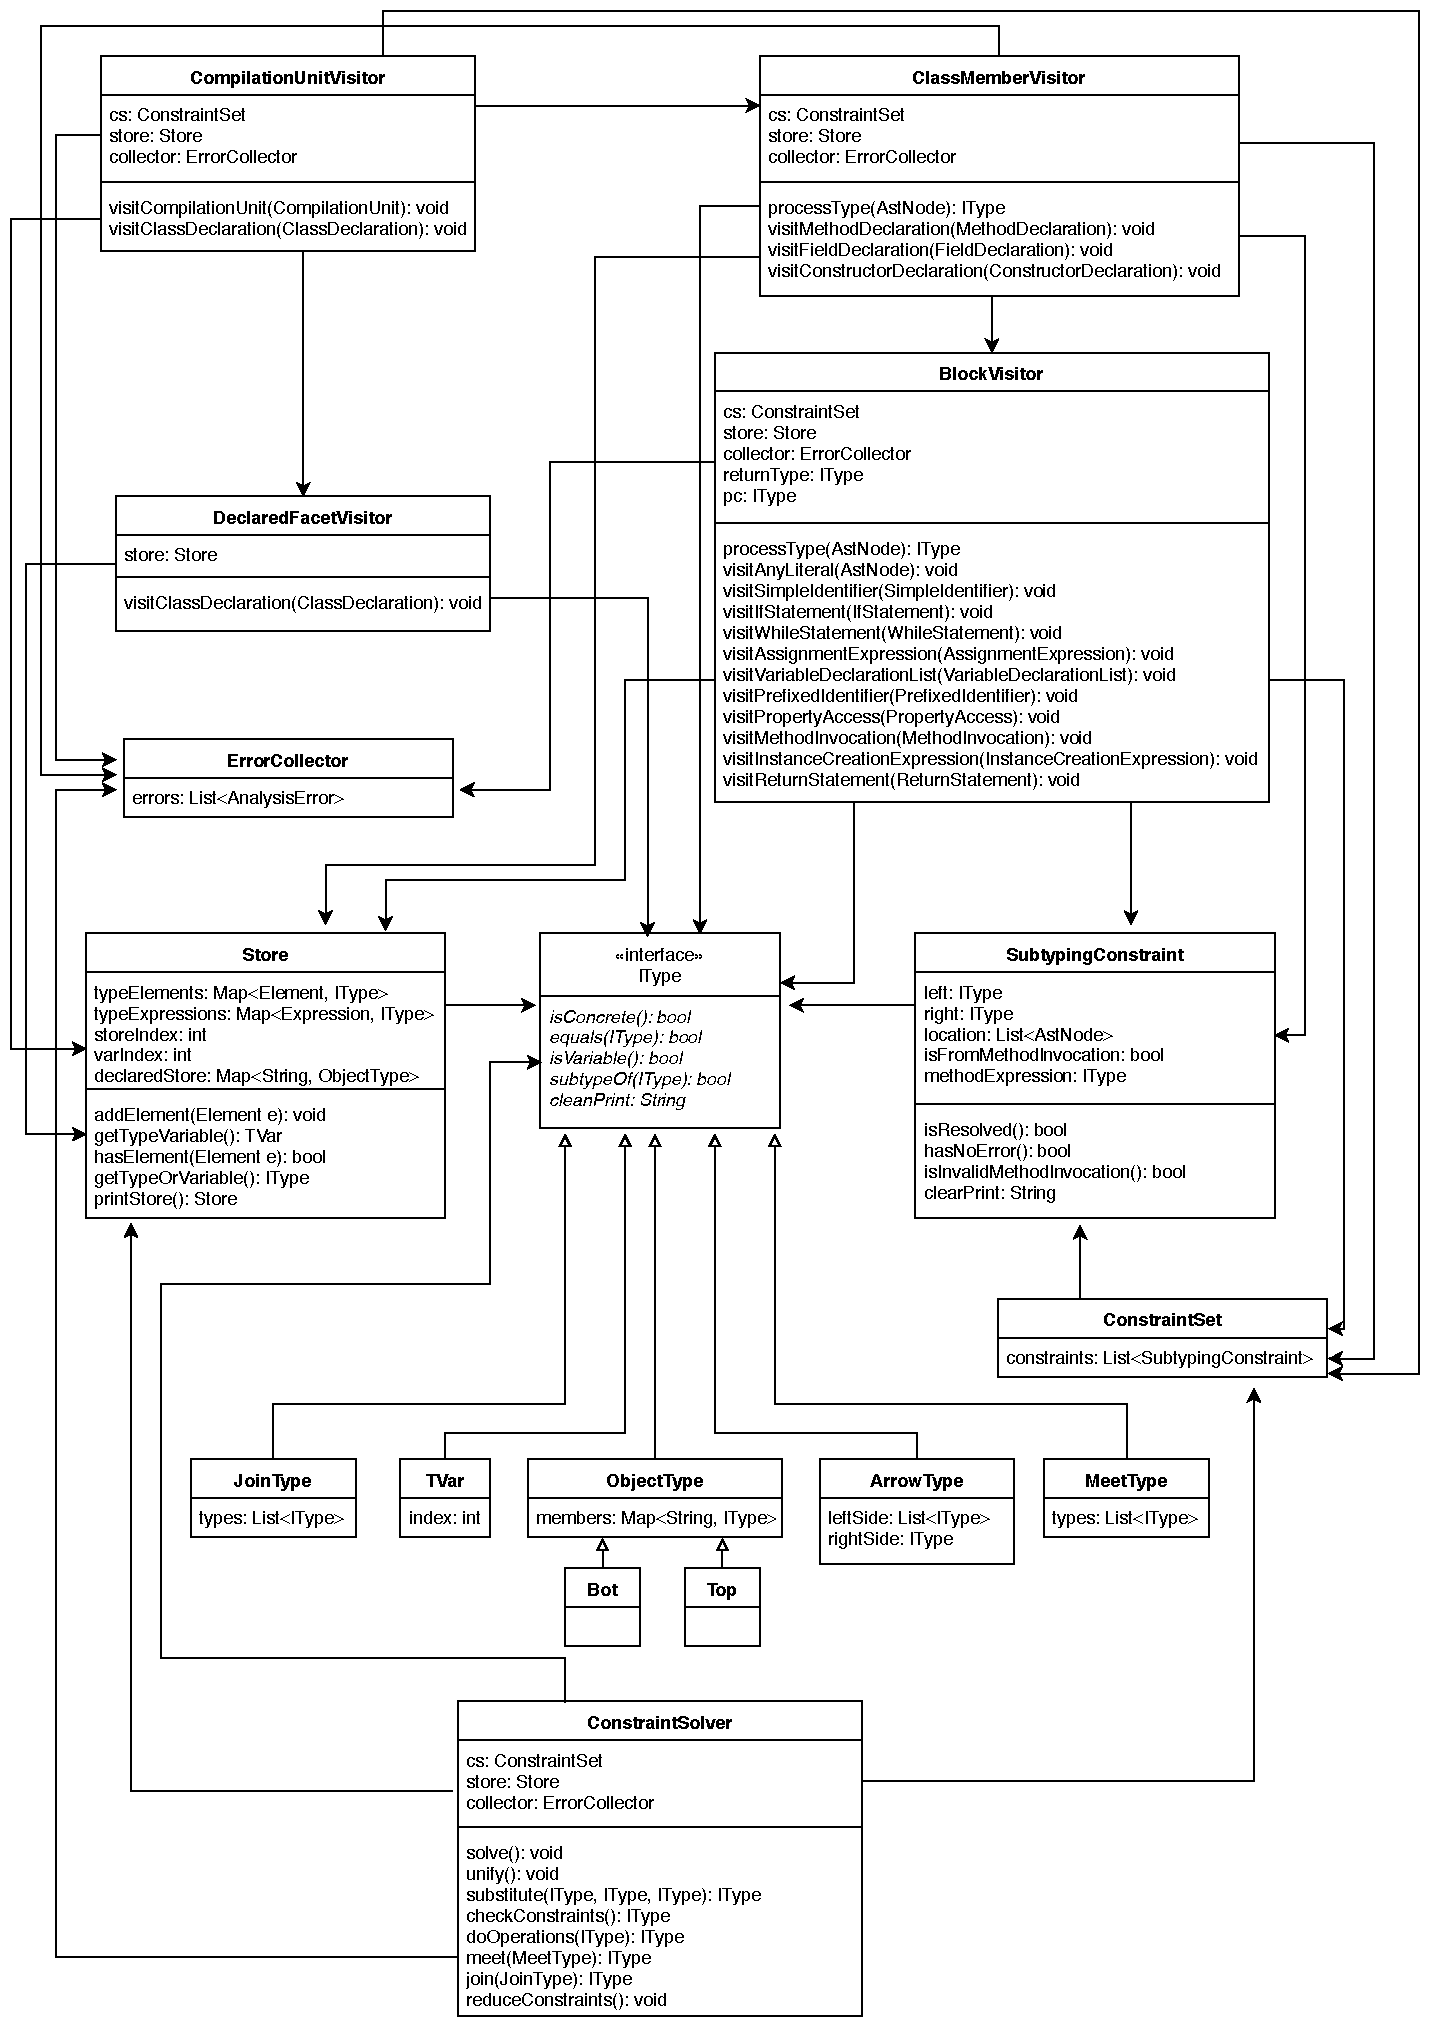
\includegraphics[width=0.93\textwidth]{imagenes/others.pdf}
  \caption{Diagrama de clases de sistema de inferencia}
  \label{uml}
\end{figure}
\clearpage

\section{Implementación de plugin}
Para la implementación del plugin, se siguió el tutorial oficial de la herramienta Analyzer Plugin, presente en el repositorio de GitHub oficial del lenguaje Dart~\cite{plugin}.

La comunicación entre el plugin y el sistema de inferencia se realiza mediante la implementación de un \emph{driver}, que administra los archivos que han sido modificados y solicita los resultados del análisis de inferencia a la clase \texttt{Analyzer}, que consiste en una lista de errores. Luego de obtener el resultado, el driver notifica al servidor de análisis para que pueda desplegar los errores en el IDE. La figura \ref{seq} muestra el diagrama de la secuencia de operaciones.

\begin{figure}[ht]
  \centering
  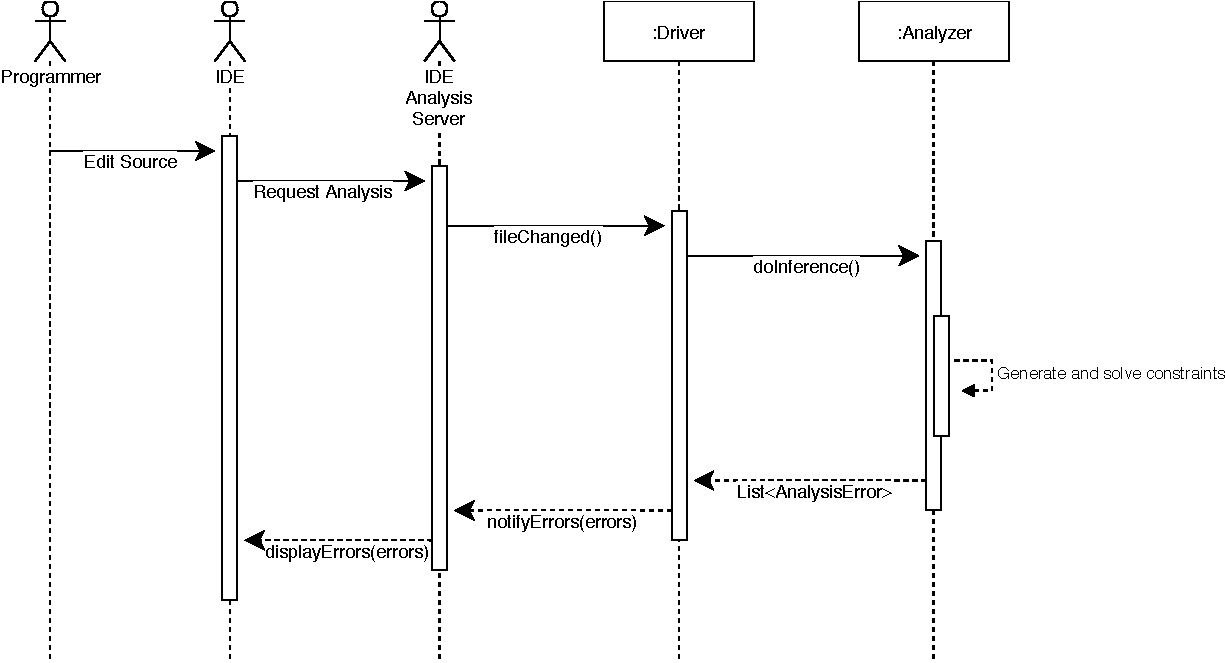
\includegraphics[width=\textwidth]{imagenes/sequence.pdf}
  \caption{Diagrama de secuencia del plugin}
  \label{seq}
\end{figure}

\subsection{Configuración del plugin}
Para activar el análisis sobre un proyecto, se debe agregar el paquete del plugin como dependencia al proyecto, y agregar el plugin al archivo de configuración del análisis del proyecto \texttt{analysis\_options.yaml}, ubicado en la raiz del proyecto.

\begin{verbatim}
  analyzer:
    plugins:
      TRNIdart:
        default_core_return: Bot
        default_core_parameter: Bot
\end{verbatim}

Las opciones \texttt{default\_core\_return} y \texttt{default\_core\_parameter} corresponden a las facetas públicas por defecto que tendrán los métodos del core de Dart.
